\section{Models for Computation}
How do you define an \textit{algorithm}? In its most basic terms, an algorithm is simply a sequence of tasks that one can perform to get a desired result. For example, in school we learn the long division method to find square root of integers. That's an algorithm.
\vspace{1em}

In the theory of computation, a computer algorithm is also similar in meaning. In 1930s the fundamental notions of the modern theory of algorithms, and thus of computation, were introduced, by Alonzo Church, Alan Turing, and other pioneers of the computer era. This work arose in response to a profound challenge laid down by the great mathematician David Hilbert in the early part of the twentieth century. Hilbert asked whether or not there existed some algorithm which could be used, in principle, to solve all the problems of mathematics. Hilbert expected that the answer to this question, sometimes known as the \textit{entscheidungsproblem}, would be yes.
\vspace{1em}

Amazingly, the answer to Hilbert’s challenge turned out to be no: there is no algorithm to solve all mathematical problems. To prove this, Church and Turing had to solve the deep problem of capturing in a mathematical definition what we mean when we use the intuitive concept of an algorithm. In so doing, they laid the foundations for the modern theory of algorithms, and consequently for the modern theory of computer science.
\vspace{1em}

Here we will describe two models of computation - Turing machines and circuit model.

\subsection{Turing machines}
The basic elements of a Turing machine are illustrated in the following figure. A Turing machine contains four main elements: (a) a \textit{program}, rather like an ordinary computer; (b) a \textit{finite state control}, which acts like a stripped-down microprocessor, coordinating the other operations of the machine; (c) a \textit{tape}, which acts like a computer memory; and (d) a \textit{read- write tape-head}, which points to the position on the tape which is currently readable or writable. We now describe each of these four elements in more detail.
\begin{figure}[h]
    \centering
    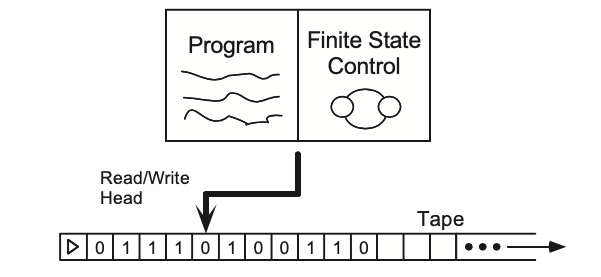
\includegraphics[width=0.70\textwidth]{turing.png}
    \caption{Main elements of a Turing machine}
\end{figure}
\vspace{1em}

The finite state control for a Turing machine consists of a finite set of internal states, $q_1,\dots, q_m$. The number $m$ is allowed to be varied; it turns out that for $m$ sufficiently large this does not affect the power of the machine in any essential way, so without loss of generality we may suppose that $m$ is some fixed constant. The best way to think of the finite state control is as a sort of microprocessor, coordinating the Turing machine’s operation. It provides temporary storage off-tape, and a central place where all processing for the machine may be done. In addition to the states $q_1 , \dots , q_m$ , there are also two special internal states, labelled $q_s$ and $q_h$. We call these the starting state and the halting state, respectively. The idea is that at the beginning of the computation, the Turing machine is in the starting state $q_s$. The execution of the computation causes the Turing machine’s internal state to change. If the computation ever finishes, the Turing machine ends up in the state $q_h$ to indicate that the machine has completed its operation.
\vspace{1em}

The Turing machine tape is a one-dimensional object, which stretches off to infinity in one direction. The tape consists of an infinite sequence of tape squares. We number the tape squares $0,1,2,3,\dots$ The tape squares each contain one symbol drawn from some alphabet, $\Gamma$, which contains a finite number of distinct symbols. For now, it will be convenient to assume that the alphabet contains four symbols, which we denote by $0, 1, b$ (the ‘blank’ symbol), and an arrow, to mark the left hand edge of the tape. Initially, the tape contains an arrow at the left hand end, a finite number of $0s$ and $1s$, and the rest of the tape contains blanks. The read-write tape-head identifies a single square on the Turing machine tape as the square that is currently being accessed by the machine.
\vspace{1em}

A \textit{program} for a Turing machine is a finite ordered list of program lines of the form $\langle q, x, q', x', s\rangle$. The first item in the program line, $q$, is a state from the set of internal states of the machine. The second item, $x$, is taken from the alphabet of symbols which may appear on the tape, $\Gamma$. The way the program works is that on each machine cycle, the Turing machine looks through the list of program lines in order, searching for a line $\langle q, x, \cdot, \cdot, \cdot \rangle$, such that the current internal state of the machine is $q$, and the symbol being read on the tape is $x$. If it doesn't find such a program line, the internal state of the machine is changed to $q_h$, and the machine halts operation. If such a line is found, then that program line is executed. Execution of a program line involves the following steps: the internal state of the machine is changed to $q'$; the symbol $x$ on the tape is overwritten by the symbol $x'$, and the tape-head moves left, right, or stands still, depending on whether $s$ is $-1$, $+1$, or $0$, respectively. The only exception to this rule is if the tape-head is at the leftmost tape square, and $s = -1$, in which case the tape-head stays put.
\vspace{1em}

It turns out that the Turing machine model of computation can be used to compute an enormous variety of functions. For example, it can be used to do all the basic arithmetical operations, to search through text represented as strings of bits on the tape, and many other interesting operations. Surprisingly, it turns out that a Turing machine can be used to simulate all the operations performed on a modern computer! Indeed, according to a thesis put forward independently by Church and by Turing, the Turing machine model of computation completely captures the notion of computing a function using an algorithm. This is known as the Church–Turing thesis:
\textit{The class of functions computable by a Turing machine corresponds exactly to the class of functions which we would naturally regard as being computable by an algorithm.}

\subsubsection*{The Universal Turing Machine}
We've described Turing machines as containing three elements which may vary from machine to machine - the initial configuration of the tape, the internal states of the finite state control, and the program for the machine. A clever idea known as the Universal Turing Machine (UTM) allows us to fix the program and finite state control once and for all, leaving the initial contents of the tape as the only part of the machine which needs to be varied.
The Universal Turing Machine (see the figure below) has the following property. Let $M$ be any Turing machine, and let $T_M$ be the Turing number associated to machine $M$. Then on input of the binary representation for $T_M$ followed by a blank, followed by any string of symbols $x$ on the remainder of the tape, the Universal Turing Machine gives as output whatever machine $M$ would have on input of $x$. Thus, the Universal Turing Machine is capable of simulating any other Turing machine!

\begin{figure}[h]
    \centering
    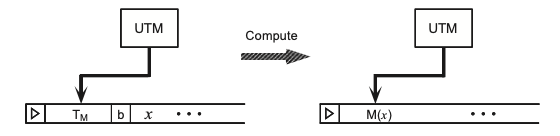
\includegraphics[width=0.70\textwidth]{UTM.png}
\end{figure}
\vspace{1em}

\subsection{Circuits}
Turing machines are rather idealized models of computing devices. Real computers are finite in size, whereas for Turing machines we assumed a computer of unbounded size. Here we investigate an alternative model of computation, the circuit model, that is equivalent to the Turing machine in terms of computational power, but is more convenient and realistic for many applications. In particular the circuit model of computation is especially important as preparation for our investigation of quantum computers.
\vspace{1em}

A circuit is made up of \textit{wires} and \textit{gates}, which carry information around, and perform simple computational tasks, respectively. More generally, a circuit may involve many input and output bits, many wires, and many logical gates. A \textit{logic gate} is a function $f : \{0,1\}^k \rightarrow \{0,1\}^l$ from some fixed number $k$ of input bits to some fixed number $l$ of output bits. 
\vspace{1em}

The following figure shows the circuit representation of the elementary logic gates.

\begin{figure}[h]
    \centering
    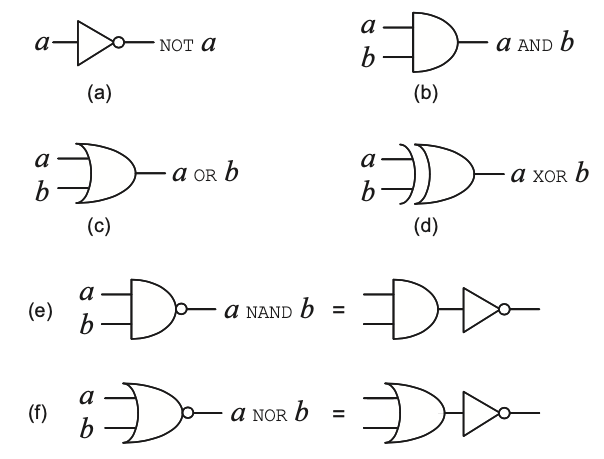
\includegraphics[width=0.70\textwidth]{logic_gates.png}
\end{figure}
\vspace{1em}

Now, let’s look at a simple example of a circuit which adds two $n$ bit integers. The basic element in this circuit is a smaller circuit known as a half-adder. A half-adder takes two bits, $x$ and $y$, as input, and outputs the sum of the bits $x \oplus y$ modulo $2$, together with a carry bit set to $1$ if $x$ and $y$ are both $1$, or $0$ otherwise.
\begin{figure}[h]
    \centering
    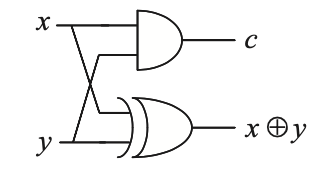
\includegraphics[width=0.35\textwidth]{half_adder.png}
    \caption{Half-adder circuit}
\end{figure}
\vspace{1em}

Two cascaded half-adders may be used to build a full-adder, as shown in the following figure. A full-adder takes as input three bits, $x$, $y$, and $c$. The bits $x$ and $y$ should be thought of as data to be added, while $c$ is a carry bit from an earlier computation. The circuit outputs two bits. One output bit is the modulo $2$ sum, $x \oplus y \oplus c$ of all three input bits. The second output bit, $c'$, is a carry bit, which is set to $1$ if two or more of the inputs is $1$, and is $0$ otherwise.
\begin{figure}[h]
    \centering
    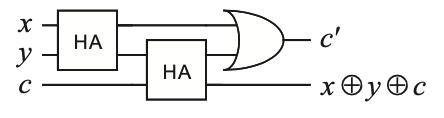
\includegraphics[width=0.55\textwidth]{full_adder.png}
    \caption{Full-adder circuit}
\end{figure}
\vspace{1em}

By cascading many of these full-adders together we obtain a circuit to add two $n$-bit
integers, as illustrated in the figure for the case $n = 3$.
\begin{figure}[h]
    \centering
    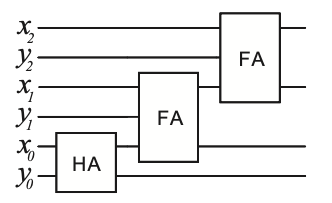
\includegraphics[width=0.45\textwidth]{3_adder.png}
    \caption{Addition circuit for two three-bit integers}
\end{figure}
\vspace{1em}

We claimed earlier that just a few fixed gates can be used to compute any function $f : \{0, 1\}^n \rightarrow \{0, 1\}^m$ whatsoever. We will now prove this for the simplified case of a function $f : \{0, 1\}^n \rightarrow \{0, 1\}$ with $n$ input bits and a single output bit. Such a function is known as a \textit{Boolean function}, and the corresponding circuit is a \textit{Boolean circuit}. The general universality proof follows immediately from the special case of Boolean functions. The proof is by induction on $n$. For $n = 1$ there are four possible functions: the identity, which has a circuit consisting of a single wire; the bit flip, which is implemented using a single $NOT$ gate; the function which replaces the input bit with a $0$, which can be obtained by $AND$ing the input with a work bit initially in the $0$ state; and the function which replaces the input with a $1$, which can be obtained by $OR$ing the input with a work bit initially in the $1$ state.
\vspace{1em}

To complete the induction, suppose that any function on $n$ bits may be computed by a circuit, and let $f$ be a function on $n + 1$ bits. Define n-bit functions $f_0$ and $f_1$ by $f_0(x_1,\dots,x_n) \equiv f(0,x_1,\dots,x_n)$ and $f_1(x_1,\dots,x_n) \equiv f(1,x_1,\dots,x_n)$. These are both $n$-bit functions, so by the inductive hypothesis there are circuits to compute these functions.
\vspace{1em}

It is now an easy matter to design a circuit which computes $f$. The circuit computes both $f_0$ and $f_1$ on the last $n$ bits of the input. Then, depending on whether the first bit of the input was a $0$ or a $1$ it outputs the appropriate answer. A circuit to do this is shown in the following figure. This completes the induction.
\begin{figure}[h]
    \centering
    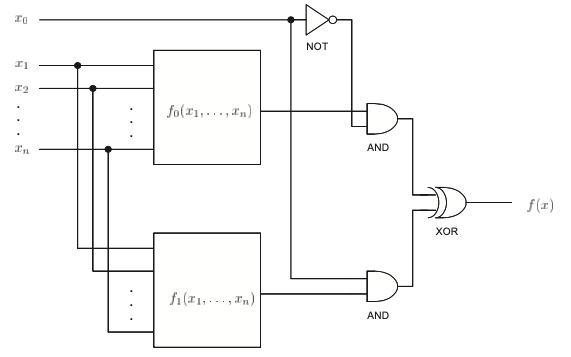
\includegraphics[width=0.70\textwidth]{induction.png}
    \caption{Circuit to compute an arbitrary function $f$ on $n + 1$ bits, assuming by induction that there are circuits to compute the $n$-bit functions $f_0$ and $f_1$.}
\end{figure}

\newpage
Let’s return from our brief quantum digression, to the properties of classical circuits. We claimed earlier that the Turing machine model is equivalent to the circuit model of computation. In what sense do we mean the two models are equivalent? On the face of it, the two models appear quite different. The unbounded nature of a Turing machine makes them more useful for abstractly specifying what it is we mean by an algorithm, while circuits more closely capture what an actual physical computer does.
\vspace{1em}

The two models are connected by introducing the notion of a \textit{uniform circuit family}. A circuit family consists of a collection of circuits, $\{C_n\}$, indexed by a positive integer $n$. The circuit $C_n$ has $n$ input bits, and may have any finite number of extra work bits, and output bits. The output of the circuit $C_n$, upon input of a number $x$ of at most $n$ bits in length, is denoted by $C_n(x)$. We require that the circuits be consistent, that is, if $m \lt n$ and $x$ is at most $m$ bits in length, then $C_m(x) = C_n(x)$. The function computed by the circuit family $\{C_n\}$ is the function $C(\cdot)$ such that if $x$ is $n$ bits in length then $C(x) = C_n(x)$. For example, consider a circuit $C_n$ that squares an $n$-bit number. This defines a family of circuits ${C_n}$ that computes the function, $C(x) = x^2$, where $x$ is any positive integer.
\vspace{1em}

In this section we saw the two models of computation and realized that the circuit model is a realistic one. In the next section we will learn about quantum circuits which are at the heart of realizing a quantum computer.